\documentclass[dvipdfmx]{beamer}
%\usepackage{indentfirst}
\usepackage{pxjahyper}
\setlength{\parindent}{11pt}
% theme
\usefonttheme{professionalfonts}
\usetheme{Madrid}
\usecolortheme{default}
\setbeamertemplate{enumerate item}[default]
\setbeamertemplate{caption}[numbered]
\setbeamertemplate{navigation symbols}{}
\usepackage[scaled]{helvet}
\renewcommand{\sfdefault}{phv}
\renewcommand{\familydefault}{\sfdefault}
\renewcommand{\kanjifamilydefault}{\gtdefault}
\setbeamertemplate{theorems}[numbered]
\definecolor{Crimson}{HTML}{dc143c}
\setbeamercolor{alerted text}{fg=Crimson}
% graphics
\usepackage{graphicx}
\usepackage{here}

% math
\usepackage{amsmath, amssymb}
\usepackage{physics}
\usepackage{mathrsfs}
\usepackage{mathtools}
\usepackage[all]{xy}
\mathversion{bold}
\definecolor{math}{HTML}{100080}
\everymath{\color{math}}

% thorem
\usepackage{amsthm}
\newtheoremstyle{break}
{\topsep}{\topsep}%
{}{}%
{\bfseries}{}%
{\newline}{}%
\theoremstyle{break}
\newtheorem{thm}{Theorem}
\newtheorem{result}[thm]{SGEの結果}

% link

\usepackage{url}
\usepackage{hyperref} 
\usepackage{xcolor}
\usepackage{pxjahyper}
\definecolor{link}{HTML}{4b0082}
\hypersetup{
	colorlinks=true,
	citecolor=link,
	linkcolor=link,
	urlcolor=orange,
}

% my command
\newcommand{\up}{\ket{\uparrow}}
\newcommand{\down}{\ket{\downarrow}}
% title
\author[T. Tanaka]{Toshiya Tanaka}
\institute[Univ. Toyama]{富山大学理学部物理学科}
\title[\textcolor{white}{SGEから始めるQM}]{数物系サーバー新歓ミニセミナー\\
Stern--Gerlachの実験から始める量子力学}

\begin{document}
\begin{frame}
		\maketitle
\end{frame}


\begin{frame}{はじめに}
		まず,聴衆のみなさんのバックグラウンドをお尋ねします.

		\begin{enumerate}
				\setbeamertemplate{items}[default]
				\item 新B1の方.\label{num:b1}
				\item 量子力学なんてなにもわからないよ,という方.\label{num:intro}
				\item ちょっとだけ勉強したことがあるよ,という方.
				\item 量子力学を完全に理解していて,冷やかしに来た方.
		\end{enumerate}

		\ref{num:b1}, \ref{num:intro}あたりの方に向けた雑談程度の講演であることはご理解ください.
\end{frame}


\begin{frame}{Introduction}
		量子力学の教科書の最初の話題は,古典論が破綻する実験事実が書かれることが多い.
		\begin{block}{伝統的なIntroduction}
		\begin{itemize}
				\item 黒体輻射\cite[\S1.1]{BN10398292}
				\item 光電効果\cite[\S1.2]{BN10398292}
				\item Compton散乱\cite[\S1.3]{BN10398292}, \cite[\S1.1, (1)]{BN0611143X}
				\item Bohrの原子模型\cite[\S1.6]{BN10398292}, \cite[\S1.1, (2)]{BN0611143X}
		\end{itemize}
		歴史的には重要であるが,破綻する古典論は統計力学・相対論など量子力学を習う段階ではしらないのが普通.
		\end{block}
		\begin{alertblock}{今回のIntroduction}
				\begin{itemize}
				\item Stern--Gerlachの実験 \cite{BC01962771}, \cite{BC08412531}
				\item 破綻する古典論は電磁気学
				\end{itemize}
		\end{alertblock}
\end{frame}


\begin{frame}{必要な古典論}
		本講演では,古典ではだめで量子論が必要であるということを感覚的に
		理解することが目的である.そのために必要な古典論の感覚を共有したい.

		\begin{columns}
				\begin{column}{0.7\textwidth}
						\begin{itemize}
								\item 電流は電子の流れであると考える.
								\item 電流のループがあると磁気モーメント$\vec{\mu}$が発生する.
								\item これをz方向の磁場$\vec{B}={}^{t}(0, 0, B_z)$の中に入れると,力$\vec{\nabla}(\vec{\mu}\cdot\vec{B})$を受ける.
								\item とにかく,力を受けること,それが内積で与えられることが大事.
								\item 内積なので,$\vec{\mu}$と$\vec{B}$のなす角$\theta\in[0, 2\pi)$による.
								\item $\theta=0$のときに受ける力の大きさを$F$とすると,$\theta$の値によって$-F$から$F$の力が考えられる.
						\end{itemize}
				\end{column}
				\begin{column}{0.3\textwidth}
						fig
				\end{column}
		\end{columns}
\end{frame}


\begin{frame}{SGEの装置}
		\begin{columns}
		\begin{column}{0.6\textwidth}
		\begin{figure}[t]
				\centering
				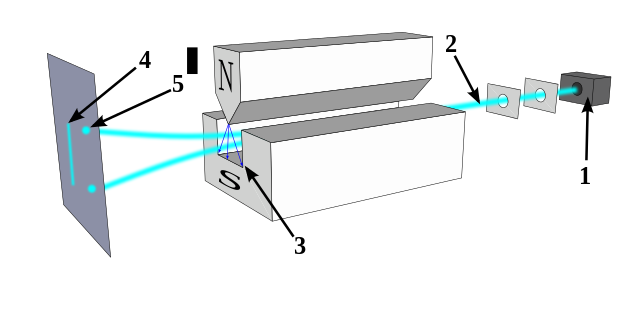
\includegraphics[keepaspectratio, scale=0.3]{./img/sg.png}
				\caption{SGの実験装置.\href{https://en.wikipedia.org/wiki/Stern\%E2\%80\%93Gerlach_experiment}{Wikipedia}より拝借.}
		\end{figure}
		\end{column}
		\begin{column}{0.4\textwidth}
		\begin{enumerate}[SG1]
				\setbeamertemplate{items}[default]
				\item 電子発射装置
				\item 電子線
				\item 磁場\label{sge_dev}
				\item 古典論からの予測\label{sge_cl}
				\item 実験結果\label{sge_qm}
		\end{enumerate}
		\end{column}
		\end{columns}
		\begin{result}\label{sgx}
				\begin{itemize}
						\item 前述した古典論からは,角度$\theta$に応じて連続的に分布する.(SG\ref{sge_cl})
						\item 実際は\alert{上下二点のみ}に\alert{等しい強度}で現れる.(SG\ref{sge_qm})
				\end{itemize}
		\end{result}
		この電子は二種類に分類できて,上の点にゆくものを$\up$,下の点にゆくものを$\down$と書くことにする.
\end{frame}


\begin{frame}[allowframebreaks]
		\begin{result}
				同じ設定で装置(SG\ref{sge_dev})を90度傾け,x方向の測定,y方向の測定,また,どれでもない斜めの方向の測定を行う.
				
				このとき,結果\ref{sgx}と同様に測定した方向に二点に分かれる.
		\end{result}
		最初にz軸と名付けるのは我々の勝手だから,どの方向を選んでも同じなのは当然のように思うが,古典的にz方向に決まった磁気モーメントを持っているわけではないということである.
		\begin{result}
				装置を二つ用意して,z方向の測定を行った後$\up$だったものに対して,再びz方向の測定を行うと,$\up$しか観測できない.$\down$に関しても同様.
		\end{result}
		\begin{result}
				装置を二つ用意して,z方向の測定を行った後$\up$だったものに対して,x方向の測定をおこなうことを考える.
				このとき,電子はx方向に二点に分かれる.これに名前をつけて,$\ket{\rightarrow}$, $\ket{\leftarrow}$と呼ぶことにする.

				$\down$, y方向に関しても同様.
		\end{result}
		x方向の測定とz方向の測定は関係しないことがわかる.

		\begin{result}
				装置を三つ用意して,z方向の測定を行った後$\up$だったものに対して,x方向の測定を行う.この測定で$\ket{\rightarrow}$だったものに対して再びz方向の測定を行うと電子は二点に分かれる.

				ややこしいので簡単に図にすると次のようになる.
		\begin{align*}
				\xymatrix@R=2pt{
						& & \up\\
						&\ket{\rightarrow}\ar[ru]\ar[rd] & \\
						& & \down\\
						\up\ar[rdd]\ar[ruu] & & \\
						& & \up\\
						&\ket{\leftarrow}\ar[ru]\ar[rd] & \\
						& & \down
				}
		\end{align*}
		\end{result}
\end{frame}
\begin{frame}[allowframebreaks]{参考文献}
		\beamertemplatetextbibitems
		\bibliography{booklist}
		\bibliographystyle{jbeta}
\end{frame}
\end{document}

